\part{衍射原理及其相关}

\section{什么是衍射}

\begin{slide}
    \begin{figure}[t]
        \centering
        \caption{红色激光的圆孔衍射图样}
        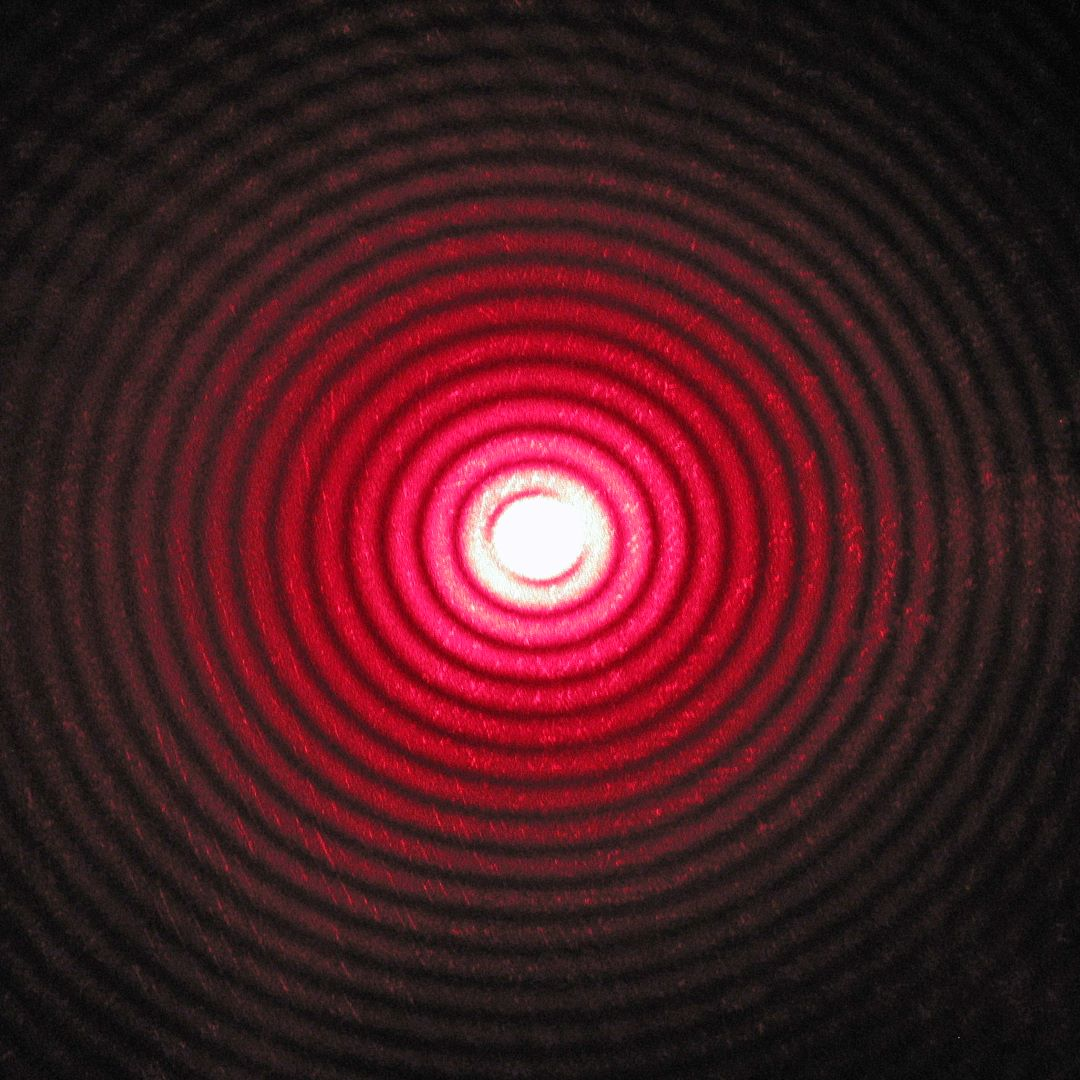
\includegraphics[height=4cm, width=4cm]{pictures/Laser_Interference.jpg}
    \end{figure}
    \textbf{波在穿过狭缝、小孔或圆盘之类的障碍物后会发生不同程度的弯散传播}，假设将一个障碍物置放在光源和观察屏之间，则会有光亮区域与阴暗区域出现于观察屏，且这些区域的边界并不锐利，是一种明暗相间的复杂图样，这种现象称为衍射
\end{slide}

\section{衍射和干涉的区别}

\begin{slide}
    \definecolor{shadecolor}{RGB}{240,248,255}
    \begin{shaded}
        \kaishu “没有人能够令人满意地定义干涉和衍射的区别。这只是术语用途的问题，其实二者在物理上并没有什么特别的、重要的区别。”\\
        \rightline{——Richard Feynman}
    \end{shaded}
    \begin{itemize}
        \item 只有少数的波源(例如两个的时候)，我们称这现象为“干涉（Interference）”，例如杨氏双缝实验
        \item 当大量波源存在时，对应的过程被称作是“衍射（Diffraction）”，特指波遇到障碍物时偏离原来直线传播的物理现象
        \item 在实际情况中，衍射和干涉往往是同时出现的
        \item 干涉是有限多个波束“相加”的结果，而衍射则是无限多个波束“积分”的结果
    \end{itemize}
\end{slide}

\section{衍射的研究历史}

\begin{slide}
    \definecolor{shadecolor}{RGB}{240,248,255}
    \begin{shaded}
        {\kaishu “光不仅会沿直线传播、折射和反射，还能够以第四种方式传播，即通过衍射的形式传播。”\\
            \rightline{——Francesco Grimaldi}
        }
    \end{shaded}
    \begin{itemize}
        \item 光的衍射效应最早由Francesco Grimaldi发现并加以描述（发表于1665年），他也是“衍射”一词的创始人
        \item Newton对这些现象进行了研究，他认为光线发生了弯曲，解释为光粒子移动于以太所产生的局部波造成
        \item Thomas Young进行了一项非常著名的实验这项实验展示了两条紧密相邻的狭缝造成的干涉现象，并进一步推测光一定具有波动的性质
    \end{itemize}
\end{slide}

\begin{slide}
    \textbf{Thomas Young的双缝实验}
    \begin{figure}[t]
        \centering
        \caption{双狭缝成像示意图}
        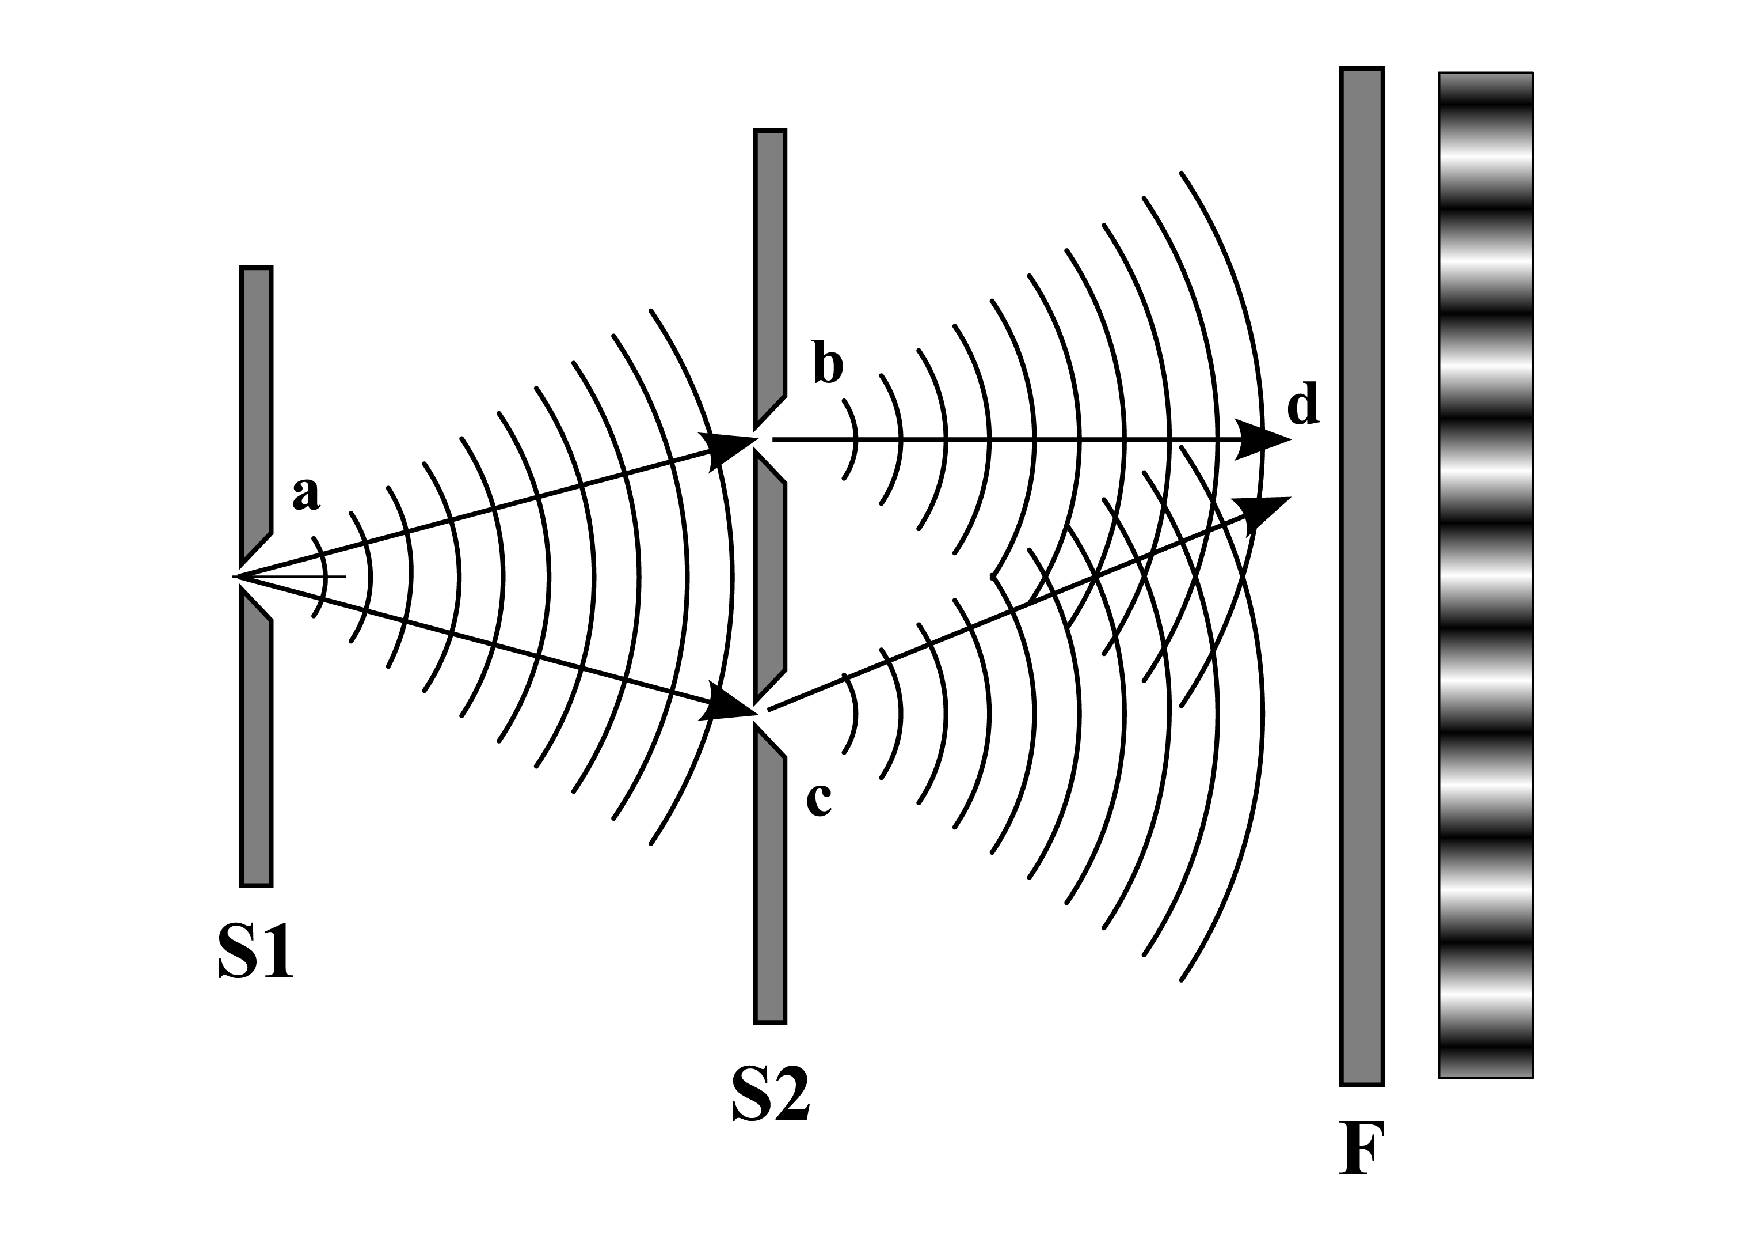
\includegraphics[height=4cm, width=5cm]{pictures/Double-slit.pdf}
    \end{figure}
    如图所示，将激光、钠黄光一类的相干光束照射到一块刻有两条狭缝的不透明板，通过狭缝的光束会抵达照相胶片或某种探测屏，从记录于照相胶片或某种探测屏的辐照度数据，可以分析得到光的波动性质
\end{slide}

\begin{slide}
    \textbf{Thomas Young的双缝实验}
    \begin{figure}[t]
        \centering
        \caption{单狭缝与双狭缝干涉实验}
        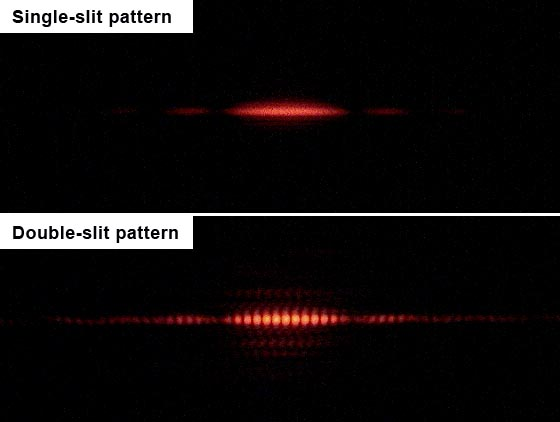
\includegraphics[height=3cm, width=4.5cm]{pictures/Single_slit_and_double_slit.jpg}
    \end{figure}
    在做单缝实验时，只有一条狭缝是开放的。单缝衍射图样（上）有一个主光带和两旁较暗淡的边光带，也可以在双缝的干涉图样看到。但是，双缝衍射图样（下）显示出两倍的光强度，而且还出现了许多小干涉条纹。

    这种图样只能用光波动说的相长干涉和相消干涉来解释，而不是用光微粒说的简单数量相加法。
\end{slide}

\begin{slide}
    \definecolor{shadecolor}{RGB}{240,248,255}
    \begin{shaded}
        {\kaishu “这样，我就展示了人们能够通过何种方式来构想光以球面波连续不断地传播出去$\cdots\cdots$”\\
            \rightline{——Augustin Fresnel}
        }
    \end{shaded}
    \begin{itemize}
        \item Fresnel则对Thomas Young的实验做了更多详细的计算研究，支持了光的波动说
        \item 作为反对光波动说的代表，Poisson提出，如果Fresnel声称的结论是正确的，那么当光射向一个球的时候，将会在球后面阴影区域的中心找到亮斑。
        \item 法国科学院的评审委员会安排了上述实验，并发现了位于阴影区域中心的亮斑，进一步证明了波动说的正确性
    \end{itemize}
\end{slide}

\begin{slide}
    \textbf{Poisson亮斑}
    \begin{itemize}
        \item 观看Poisson亮斑实验视频
        \item \url{https://www.bilibili.com/video/BV1M4411t7HK}
    \end{itemize}
\end{slide}

\section{衍射的物理原理}

\begin{slide}
    \begin{itemize}
        \item 惠更斯（Huygens）于17世纪提出: 可以把波前的每一点考虑为次波（球面波）的点波源，这些次波互相干涉，叠加形成新的波前
        \item 1818年左右，菲涅耳在巴黎科学院关于解释衍射现象的有奖竞赛中，吸收了惠更斯“次波”的思想，并加入了他对于干涉现象的理解，使上述理论得以发展和完善
        \item \textbf{惠更斯\symbol{"2E3A}菲涅耳原理}:波前上的每个面元可以看为次波源，它们向四周发射次波；波场中任一场点的扰动，是所有次波源所贡献的次级扰动的相干叠加
        \item 相干叠加并非简单的代数求和，而必须虑及这些波各自的相对相位以及振动方向
    \end{itemize}
\end{slide}

\begin{slide}
    一般化的波动方程为：
    \begin{equation}
        \nabla^2 \Psi -\ \frac{1}{c^2}\ \frac{\partial^2 \Psi}{\partial t^2 }
        = - F(\bm{r},t)
    \end{equation}
    这里$\Psi$为标量波，$F(\bm{r},t)$为波前上所有(次)波源分布（因为考虑成标量波所以略掉了倾斜因子$f(\theta,\theta_0)=\dfrac{\theta+\theta_0}{2}$的影响）\\~\\
    假设所有波源只含频率为$\omega$的本征模式，即$F(\bm{r},t)=f(\bm{r})e^{-i\omega t}$，则(1)可化为不含时波动方程
    \begin{equation}
        \nabla^2 \psi + k^2 \psi = -  f(\bm{r})
    \end{equation}
    这里$k=\omega/c$是波矢大小，$\psi(\bm{r})$是波的不含时空间分布：
    $\Psi(\bm{r},t)=\psi(\bm{r})\mathrm{e}^{-i\omega t}$
\end{slide}

\begin{slide}
    (2)是典型的非齐次亥姆霍兹方程，求出对应的格林函数方程
    \begin{equation}
        \nabla^2 G(\bm{r},\bm{r}') + k^2 G(\bm{r},\bm{r}')
        = -\delta(\bm{r}-\bm{r}')
    \end{equation}

    解出对应的格林函数后，应用格林公式可以算得
    \begin{equation}
        \psi(\bm{r}) = \int\limits_{\mathbb{V}}f(\bm{r}')G(\bm{r},\bm{r}') \mathrm{d}^3\bm{r}'
    \end{equation}
    所以现在关键在于解决(2)
    \begin{equation*}
        \nabla^2 G(\bm{r},\bm{r}') + k^2 G(\bm{r},\bm{r}')
        = -\delta(\bm{r}-\bm{r}')
    \end{equation*}
\end{slide}

\begin{slide}
    一般采用球坐标求解格林函数，如下
    \begin{equation}
        \frac{1}{R} \frac {\mathrm{d}^2}{\mathrm{d} R^2} (RG) +k^2 G
        = -\delta(\bm{R})
    \end{equation}
    可以试探出球面波解
    \begin{equation}
        G(\bm{R},\bm{O}) = \frac{e^{ikR}}{4\pi R}
    \end{equation}
    换回一般性的坐标有
    \begin{equation}
        G(\bm{r},\bm{r}') = \frac{e^{ik |\bm{r}-\bm{r}' | }}{4\pi |\bm{r}-\bm{r}' |}
    \end{equation}
    则对于整个面波前的积分有
    \begin{equation}
        \psi= \int\limits_{\mathbb{V}} f(\bm{r}')G(\bm{r},\bm{r}')d^3\bm{r}' =\int\limits_{\mathbb{S}} f_s(\bm{r}')\frac{e^{i k |\bm{r}- \bm{r}'|}}{4\pi |\bm{r}-\bm{r}'|}d\sigma'
    \end{equation}
\end{slide}

\section{推广到基尔霍夫衍射公式}

\begin{slide}
    \begin{itemize}
        \item 实验中没有出现次波源贡献叠加后逆初始方向传播的波，引入倾斜因子$\dfrac{1+\cos{\chi}}{2}$
    \end{itemize}
    \begin{figure}[b]
        \centering
        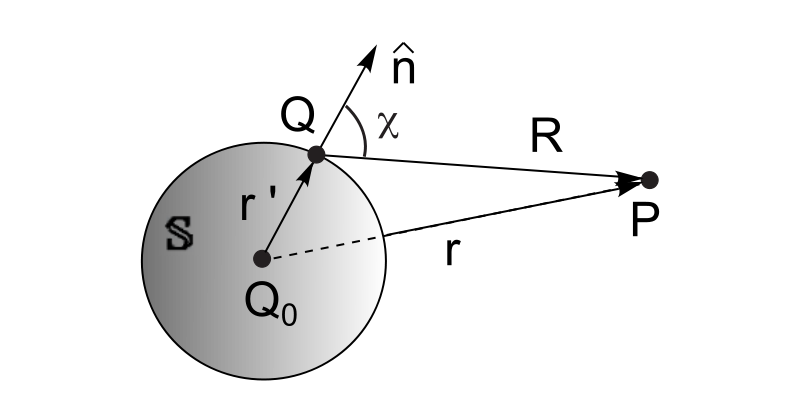
\includegraphics[height=4.5cm, width=8cm]{pictures/Fresnel-Kirchhoff_Diffraction_Formula_spherical_wavefront.png}
        \caption{倾斜因子示意图}
    \end{figure}
\end{slide}

\begin{slide}
    基尔霍夫(Kirchoff)通过求解格林第二公式给出了解的严格推导
    \begin{equation}
        \psi(\bm{r})=\frac{1}{4\pi}\oint\limits_{\mathbb{S}}\left[\psi(\bm{r}')\nabla'\left( \frac{e^{ikR}}{R} \right)-\left( \frac{e^{ikR}}{R} \right)\nabla'\psi(\bm{r}')\right]\cdot\mathrm{d}\bm{S}'
    \end{equation}
    在$k>>1/R$、$k>>1/r^{\prime}$条件下，推导出了$-\dfrac{i}{\lambda}$因子
    \begin{equation}
        \psi(\bm{r}) =-\ \frac{i}{\lambda}\oint\limits_{\mathbb{S}}\left(\frac{e^{ikR}}{R}\right)\frac{\cos{\theta_0+\cos{\theta}}}{2}\psi(\bm{r}')\mathrm{d}S'
    \end{equation}
    这里满足$\dfrac{a^2}{L\lambda}\geq 1$，$a$为圆孔半径，$\lambda$为入射波的波长，$L$为观察屏距离圆孔、狭缝等衍射物体的距离，故也被称为\textbf{菲涅耳衍射}，它是衍射的近场近似
\end{slide}

\section{夫琅和费衍射}

\begin{slide}
    \begin{itemize}
        \item 当$\dfrac{a^2}{L\lambda}\ll1$时，被称为\textbf{夫琅和费衍射}，它是衍射的远场近似
        \item 最典型的夫琅和费衍射就是单缝衍射
    \end{itemize}
    \begin{figure}[b]
        \centering
        \caption{单缝衍射}
        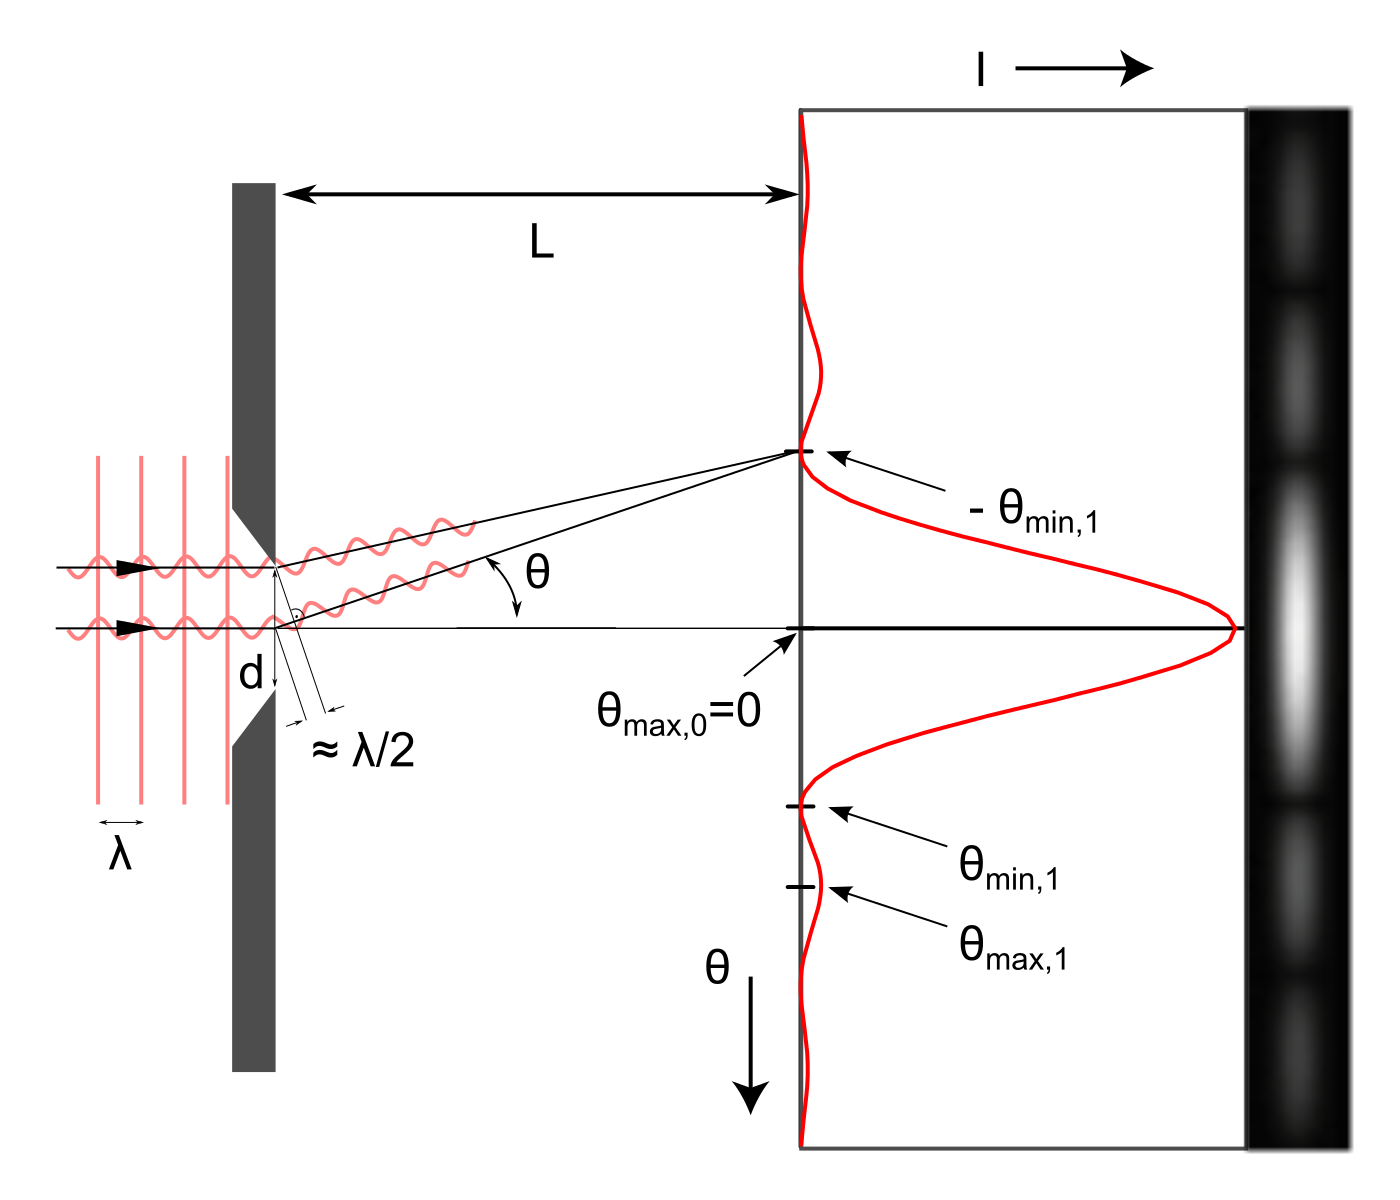
\includegraphics[height=4.8cm, width=6.4cm]{pictures/Single_Slit_Diffraction_First_Minimum.png}
    \end{figure}
\end{slide}

\begin{slide}
    \textbf{夫琅和费衍射光栅}
    \small
    \begin{itemize}
        \item 衍射光栅是狭缝按照一定规律分布的光学装置，它能够调整入射光的相位、振幅等属性，使透过它的光发生衍射、干涉
        \item 所有衍射光栅的$m$级极大衍射角$\theta_m$满足下列光栅方程
              \begin{equation}
                  d\left( \sin{\theta_m} + \sin{\theta_i} \right) = m \lambda
              \end{equation}
        \item 衍射光栅的强度分布$P$是衍射因子和干涉因子的乘积，即$P = D(\theta)\cdot I(\theta)$,其中衍射因子
              \begin{equation}
                  D= \frac{ \sin(\pi\cdot d\cdot\sin(\theta)/\lambda)^2\cdot\lambda^2}{(\pi^2\cdot d^2\cdot\sin(\theta)^2)}
              \end{equation}
              干涉因子
              \begin{equation}
                  I= \frac{\sin(\pi\cdot a\cdot\sin(\theta)\cdot N/\lambda)^2}{(N^2\cdot\sin(\pi\cdot a\cdot\sin(\theta)/\lambda)^2)}
              \end{equation}
    \end{itemize}
    \begin{figure}[b]
        \centering
        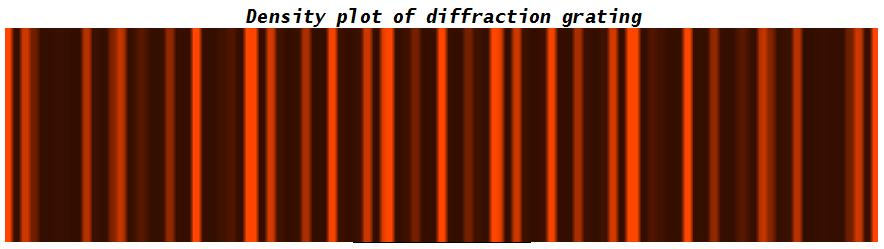
\includegraphics[height=1.6cm, width=6.4cm]{pictures/Density_plot_of_diffraction_grating.jpg}
    \end{figure}
\end{slide}

\section{布拉格衍射}

\begin{slide}
    \small
    \begin{itemize}
        \item 晶体具有周期性的物质结构。由于在这种周期性结构中，原子间距为$10^{-10}$米数量级，因此它可以作为波的衍射光栅
        \item 同相位的入射波经过不同晶面，在晶格原子处发生衍射后，从而产生干涉相长或干涉相消，这就形成了布拉格衍射
        \item 根据布拉格定律，干涉加强位置所满足的条件为
              \begin{equation}
                  m\lambda=2d\sin{\theta}
              \end{equation}
              这里$\lambda$为波长，$d$为晶面距离，$\theta$为衍射角，$m$为衍射级数
    \end{itemize}
    \begin{figure}[b]
        \centering
        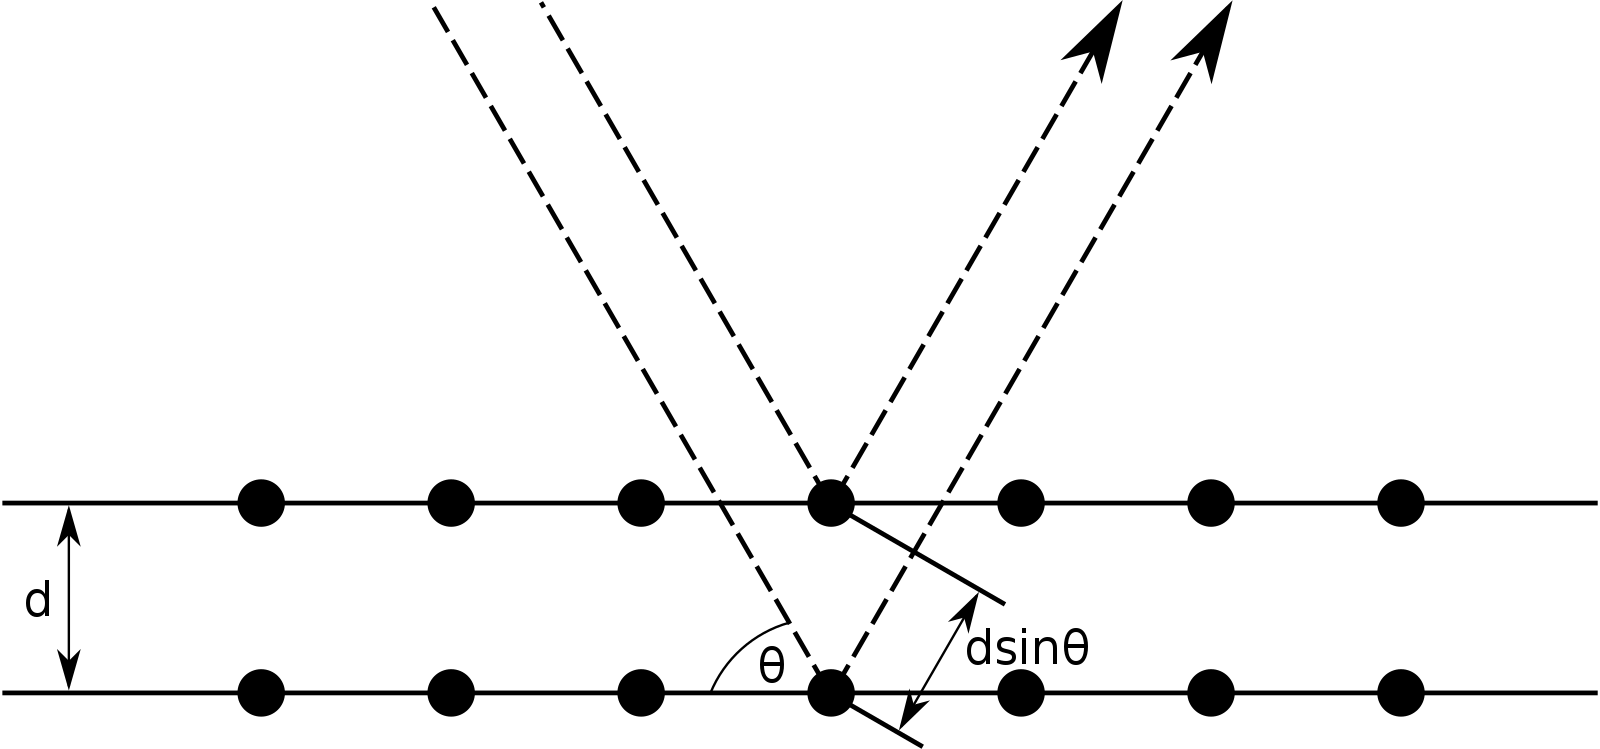
\includegraphics[height=3cm, width=6cm]{pictures/BraggPlaneDiffraction.png}
    \end{figure}
\end{slide}

\section{单缝衍射中的不确定性}

\begin{slide}
    \begin{itemize}
        \item 根据单狭缝衍射公式，从中央极大值位置（最大波强度之点）到第一个零点（零波强度之点）的夹角$\theta$ 为$\sin\theta= \lambda/w$
        \item 给定平面波的波长，狭缝越窄，衍射现象越宽阔，$\theta$ 越大；狭缝越宽，衍射现象越窄缩，$\theta$ 越小
        \item 当粒子穿过狭缝之前，在粒子前进的方向（$x$方向）的动量为$p$，在$y$方向的动量$p_{y}$是零。穿过狭缝时，粒子的动量经衍射发生变化。$p_{y}$的不确定性$\Delta p_{y}$大约是$\Delta p_y\approx p\sin\theta\approx p\lambda/w$
    \end{itemize}
    \begin{figure}[b]
        \centering
        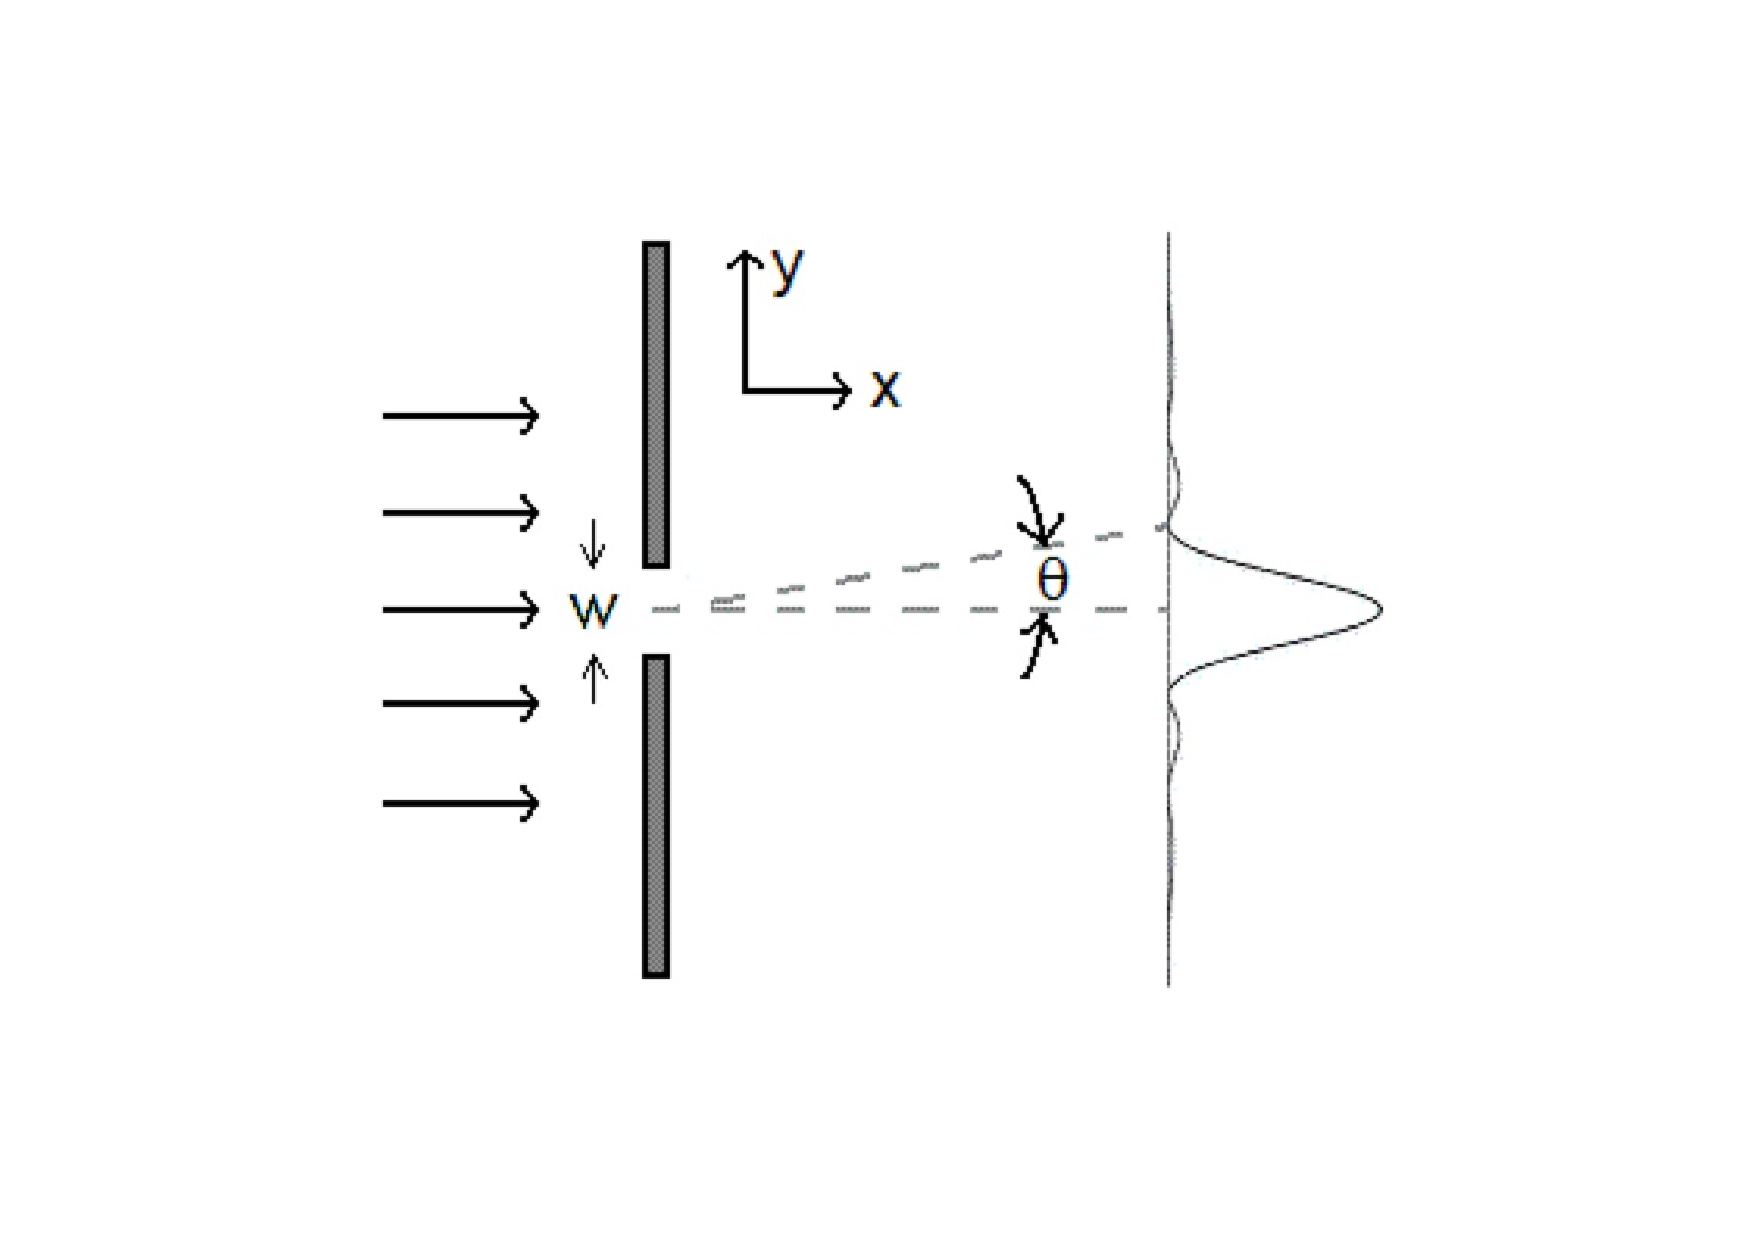
\includegraphics[height=4cm, width=6cm]{pictures/SingleSlitDiffraction.pdf}
    \end{figure}
\end{slide}

\begin{slide}
    \small
    \begin{itemize}
        \item 当粒子穿过狭缝时，其位置不确定性$\Delta y$是狭缝宽度:$\Delta y\approx w$
        \item 所以，位置不确定性与动量不确定性的乘积大约为
              \begin{equation}
                  \Delta y\Delta p_y\approx\lambda p
              \end{equation}
        \item 从德布罗意假说有$\lambda=h/p$
        \item 所以，位置不确定性与动量不确定性遵守近似式
              \begin{equation}
                  \Delta y\Delta p_y\approx h
              \end{equation}
    \end{itemize}
    \begin{figure}[b]
        \centering
        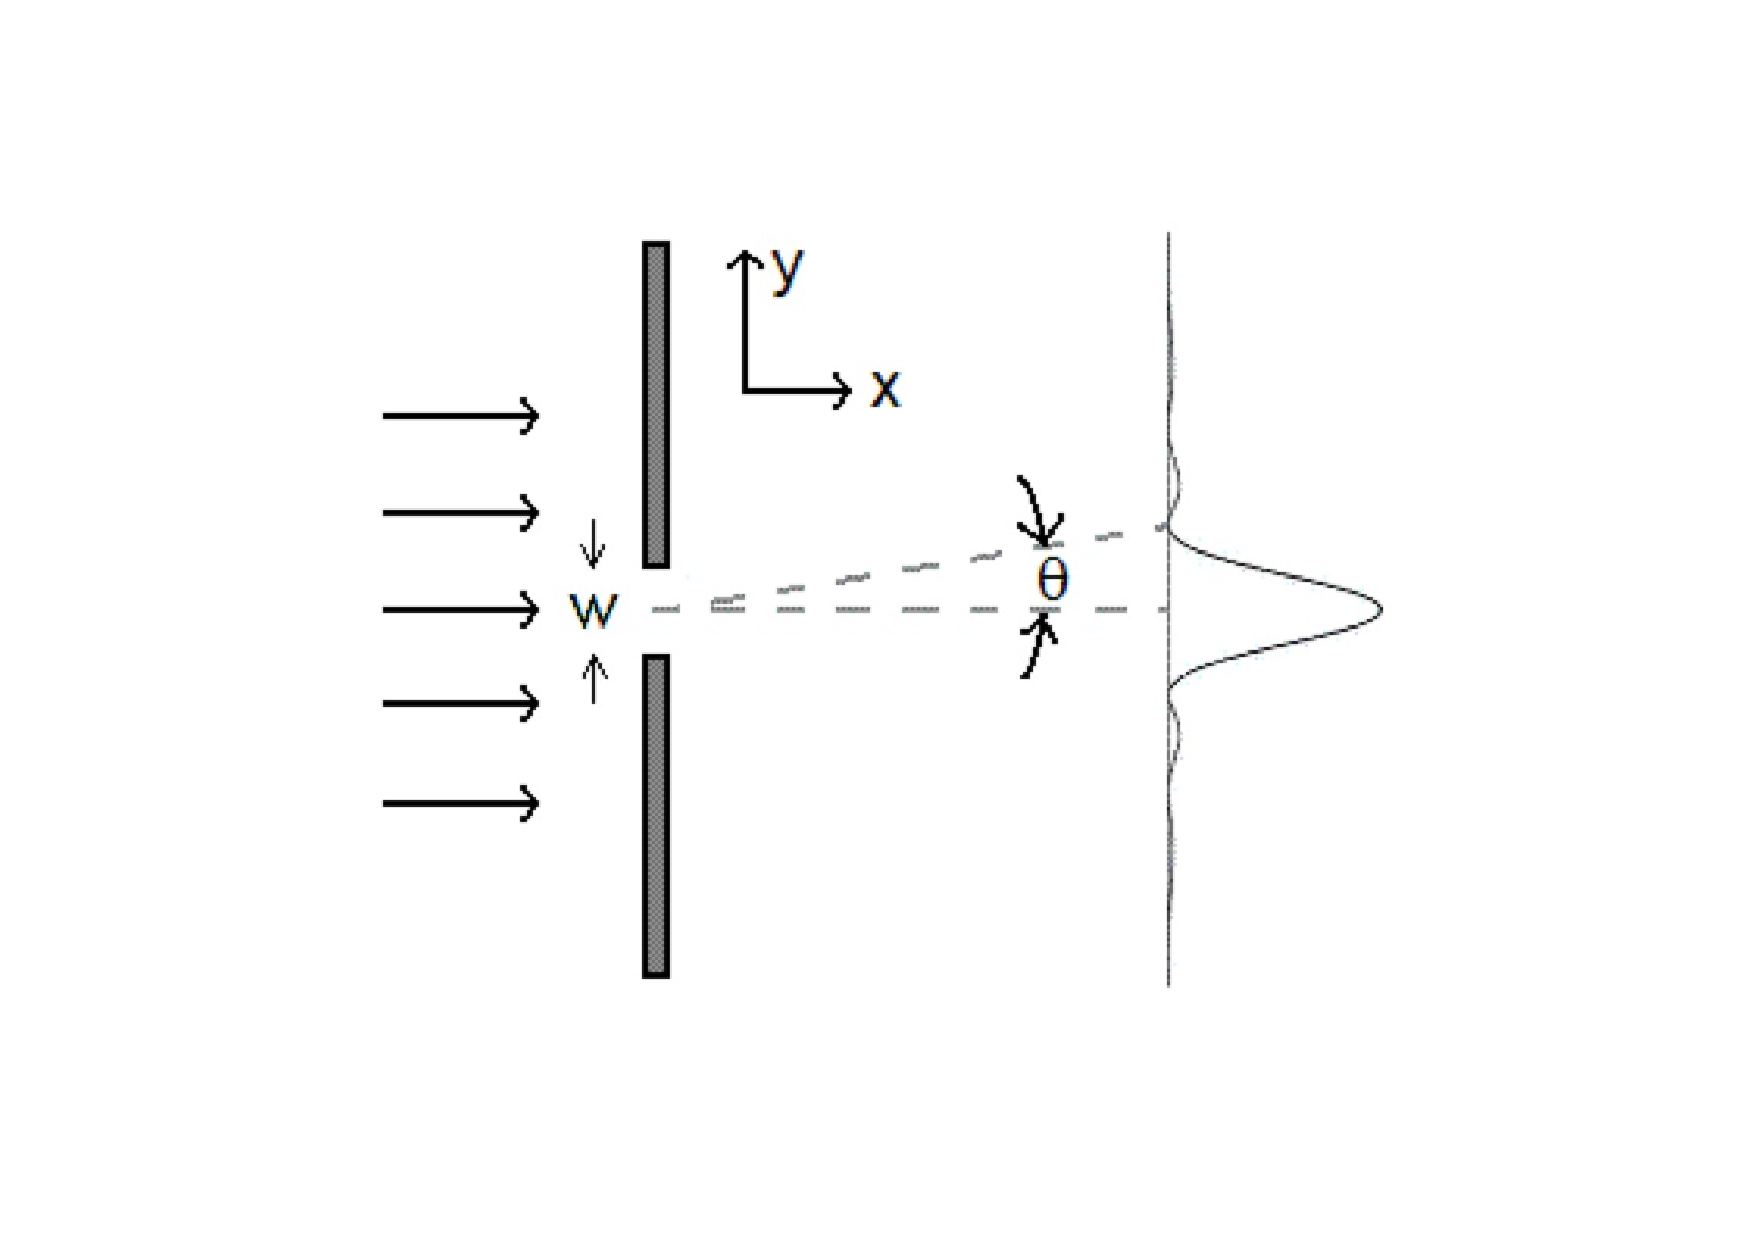
\includegraphics[height=4cm, width=6cm]{pictures/SingleSlitDiffraction.pdf}
    \end{figure}
\end{slide}

\section{衍射必要条件：相干性}

\begin{slide}
    \begin{itemize}
        \item 一束光波的相位在某段长度上是相关的，这段长度被称作是纵向相干长度，简称为“相干长度”
        \item 为了使干涉或衍射能够发生，光程差必须小于相干长度
        \item 如果采用不相干入射光，那么其中的不同波传播到给定点时的相位差将会极快地、无规则地变化，这样在观察屏上就无法形成稳定的干涉相长或干涉相消的图样，而是在这两种情况之间不断变化，以至于无法观察到明暗条纹
        \item 如果光波由扩展光源发射，则可能会出现横向的不相干
        \item 在杨氏双缝实验中，这意味着如果横向相干长度比两条狭缝的间距小，那么在观察屏上形成的图样看起来就像是两个独立单缝形成的衍射图样
        \item 在电子、中子和原子等离子的情况中，相干长度与描述粒子的波函数的空间范围有关
    \end{itemize}
\end{slide}

\stepcounter{part}
